\begin{center}
	\begin{tabular}{rp{6cm}lp{10cm}}%{rl}
		% after \\: \hline or \cline{col1-col2} \cline{col3-col4} ...
		论文地址:& \href{https://arxiv.org/abs/2010.02949}{https://arxiv.org/abs/2010.02949} \\
		源码地址:& \href{https://shalab.usc.edu/DG/}{DG} \\
		关键词:& \textbf{embedding, multimodal,  Denotation Graph} \\
		写于:& \date{2020-10-08}
	\end{tabular}
\end{center}
该论文\cite{zhang2020learning}提出了一种表征多模态(图像+文本)数据的方法。存在着大量对齐的“视觉+文本”的数据,如包含描述的图片、视频、带字幕的电影等。学习如何表示这种视觉和文本存在明显的语义联系的数据是有很大引用价值的,如通过文本搜索图片、视频,为视频/图片添加描述,通过语言查询视频/图片中的信息,可视化的问答系统等。\\
\begin{figure}[h]
	\centering
	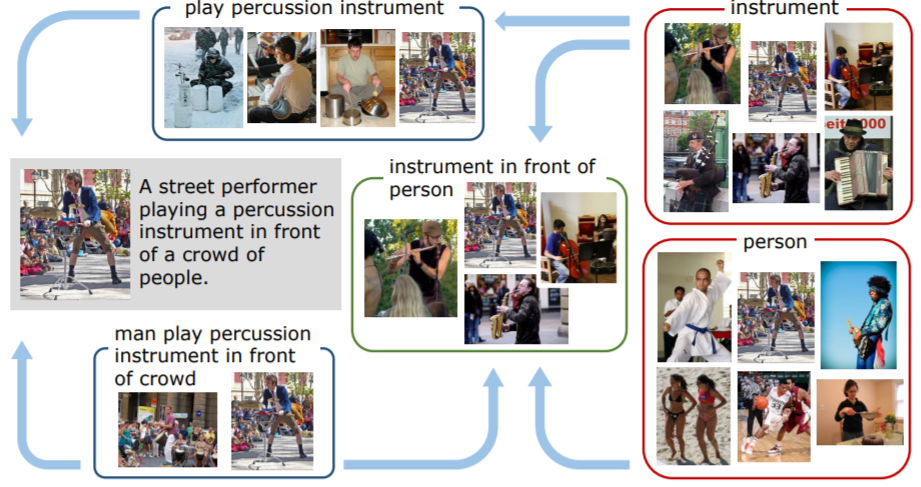
\includegraphics[width=.8\textwidth]{pics/DG.png}
	\caption{denotation graph extracted from the FLICKR30K dataset}
	\label{fig:DG}
\end{figure}
\textbf{方法}\hspace{6pt}论文中使用denotation graph(DG)\cite{young-etal-2014-image}来表示“图像+文本”的数据。该论文中的DG中每个结点包含一个文本描述和一系列与之对应的图像,图中的边是有向边,从语义上抽象的结点指向更具体地结点。如Fig.\ref{fig:DG}所示,DG中抽象的结点具有更一般的概念(如图中的person, instrument),抽象结点会指向更具体地结点(如play percussion instrument),每个结点会包含结点概念所对应的一些列图片。为什么要将文本与图像对应起来呢?论文中基于这样的一个假设:图片与文本对应的一致性有利于下游任务。在得到上述的DG(构建DG可参考\href{https://github.com/aylai/DenotationGraph}{这里}和\cite{young-etal-2014-image})后,在DG基础上学习图片和文本地表征。